%%%%%%%%%%%%%%%%%%%%%%%%%%%%%%%%%%%%%%%%%
% Wenneker Article
% LaTeX Template
% Version 2.0 (28/2/17)
%
% This template was downloaded from:
% http://www.LaTeXTemplates.com
%
% Authors:
% Vel (vel@LaTeXTemplates.com)
% Frits Wenneker
%
% License:
% CC BY-NC-SA 3.0 (http://creativecommons.org/licenses/by-nc-sa/3.0/)
%
%%%%%%%%%%%%%%%%%%%%%%%%%%%%%%%%%%%%%%%%%

%----------------------------------------------------------------------------------------
%	PACKAGES AND OTHER DOCUMENT CONFIGURATIONS
%----------------------------------------------------------------------------------------

\documentclass[10pt, a4paper, twocolumn]{article} % 10pt font size (11 and 12 also possible), A4 paper (letterpaper for US letter) and two column layout (remove for one column)

%%%%%%%%%%%%%%%%%%%%%%%%%%%%%%%%%%%%%%%%%
% Wenneker Article
% Structure Specification File
% Version 1.0 (28/2/17)
%
% This file originates from:
% http://www.LaTeXTemplates.com
%
% Authors:
% Frits Wenneker
% Vel (vel@LaTeXTemplates.com)
%
% License:
% CC BY-NC-SA 3.0 (http://creativecommons.org/licenses/by-nc-sa/3.0/)
%
%%%%%%%%%%%%%%%%%%%%%%%%%%%%%%%%%%%%%%%%%

%----------------------------------------------------------------------------------------
%	PACKAGES AND OTHER DOCUMENT CONFIGURATIONS
%----------------------------------------------------------------------------------------

\usepackage[english]{babel} % English language hyphenation

\usepackage{microtype} % Better typography

\usepackage{amsmath,amsfonts,amsthm} % Math packages for equations

\usepackage[svgnames]{xcolor} % Enabling colors by their 'svgnames'

\usepackage[hang, small, labelfont=bf, up, textfont=it]{caption} % Custom captions under/above tables and figures

\usepackage{booktabs} % Horizontal rules in tables

\usepackage{lastpage} % Used to determine the number of pages in the document (for "Page X of Total")

\usepackage{graphicx} % Required for adding images

\usepackage{enumitem} % Required for customising lists
\setlist{noitemsep} % Remove spacing between bullet/numbered list elements

\usepackage{sectsty} % Enables custom section titles
\allsectionsfont{\usefont{OT1}{phv}{b}{n}} % Change the font of all section commands (Helvetica)

 \usepackage{setspace} \doublespacing 
\usepackage[switch]{lineno} 

% \usepackage{amsmath}
% \usepackage{breqn}
\usepackage{mathtools}

%----------------------------------------------------------------------------------------
%	MARGINS AND SPACING
%----------------------------------------------------------------------------------------

\usepackage{geometry} % Required for adjusting page dimensions

\geometry{
	top=1cm, % Top margin
	bottom=1.5cm, % Bottom margin
	left=2cm, % Left margin
	right=2cm, % Right margin
	includehead, % Include space for a header
	includefoot, % Include space for a footer
	%showframe, % Uncomment to show how the type block is set on the page
}

\setlength{\columnsep}{7mm} % Column separation width

%----------------------------------------------------------------------------------------
%	FONTS
%----------------------------------------------------------------------------------------

\usepackage[T1]{fontenc} % Output font encoding for international characters
\usepackage[utf8]{inputenc} % Required for inputting international characters

\usepackage{XCharter} % Use the XCharter font

%----------------------------------------------------------------------------------------
%	HEADERS AND FOOTERS
%----------------------------------------------------------------------------------------

\usepackage{fancyhdr} % Needed to define custom headers/footers
\pagestyle{fancy} % Enables the custom headers/footers

\renewcommand{\headrulewidth}{0.0pt} % No header rule
\renewcommand{\footrulewidth}{0.4pt} % Thin footer rule

\renewcommand{\sectionmark}[1]{\markboth{#1}{}} % Removes the section number from the header when \leftmark is used

%\nouppercase\leftmark % Add this to one of the lines below if you want a section title in the header/footer

% Headers
\lhead{} % Left header
\chead{\textit{\thetitle}} % Center header - currently printing the article title
\rhead{} % Right header

% Footers
\lfoot{} % Left footer
\cfoot{} % Center footer
\rfoot{\footnotesize Page \thepage\ of \pageref{LastPage}} % Right footer, "Page 1 of 2"

\fancypagestyle{firstpage}{ % Page style for the first page with the title
	\fancyhf{}
	\renewcommand{\footrulewidth}{0pt} % Suppress footer rule
}

%----------------------------------------------------------------------------------------
%	TITLE SECTION
%----------------------------------------------------------------------------------------

\newcommand{\authorstyle}[1]{{\large\usefont{OT1}{phv}{b}{n}\color{Black}#1}} % Authors style (Helvetica)

\newcommand{\institution}[1]{{\footnotesize\usefont{OT1}{phv}{m}{sl}\color{Black}#1}} % Institutions style (Helvetica)

\usepackage{titling} % Allows custom title configuration

\newcommand{\HorRule}{\color{Black}\rule{\linewidth}{1pt}} % Defines the gold horizontal rule around the title

\pretitle{
	\vspace{-30pt} % Move the entire title section up
	\HorRule\vspace{10pt} % Horizontal rule before the title
	\fontsize{32}{36}\usefont{OT1}{phv}{b}{n}\selectfont % Helvetica
	\color{Black} % Text colour for the title and author(s)
}

\posttitle{\par\vskip 15pt} % Whitespace under the title

\preauthor{} % Anything that will appear before \author is printed

\postauthor{ % Anything that will appear after \author is printed
	\vspace{10pt} % Space before the rule
	\par\HorRule % Horizontal rule after the title
	\vspace{20pt} % Space after the title section
}

%----------------------------------------------------------------------------------------
%	ABSTRACT
%----------------------------------------------------------------------------------------

\usepackage{lettrine} % Package to accentuate the first letter of the text (lettrine)
\usepackage{fix-cm}	% Fixes the height of the lettrine

\newcommand{\initial}[1]{ % Defines the command and style for the lettrine
	\lettrine[lines=3,findent=4pt,nindent=0pt]{% Lettrine takes up 3 lines, the text to the right of it is indented 4pt and further indenting of lines 2+ is stopped
		\color{DarkGoldenrod}% Lettrine colour
		{#1}% The letter
	}{}%
}

\usepackage{xstring} % Required for string manipulation

\newcommand{\lettrineabstract}[1]{
	\StrLeft{#1}{1}[\firstletter] % Capture the first letter of the abstract for the lettrine
	\initial{\firstletter}\textbf{\StrGobbleLeft{#1}{1}} % Print the abstract with the first letter as a lettrine and the rest in bold
}

%----------------------------------------------------------------------------------------
%	BIBLIOGRAPHY
%----------------------------------------------------------------------------------------
% \usepackage{natbib}
% \bibliographystyle{molecularEcology.bst}

\usepackage[backend=biber,style=apa,natbib=true]{biblatex} % Use the bibtex backend with the authoryear citation style (which resembles APA)

\addbibresource{tellis.bib} % The filename of the bibliography

\usepackage[autostyle=true]{csquotes} % Required to generate language-dependent quotes in the bibliography
 % Specifies the document structure and loads requires packages

%----------------------------------------------------------------------------------------
%	ARTICLE INFORMATION
%----------------------------------------------------------------------------------------

\title{Joint estimation of paternity, sibships and pollen dispersal in a snapdragon hybrid zone} % The article title

\author{
	\authorstyle{Thomas James Ellis\textsuperscript{1,2,3}, David Luke Field, \textsuperscript{2,3}, Nicholas H. Barton\textsuperscript{2}} % Authors
	\newline\newline % Space before institutions
	\textsuperscript{1}\institution{Institute of Science and Technology Austria, 2234 Klosterneuburg, Austria}\\ % Institution 1
	\textsuperscript{2}\institution{Gregor Mendel Institute of Molecular Plant Sciences, Dr.-Bohr-Gasse 3, 1030 Vienna, Austria}\\ % Institution 2
	\textsuperscript{3}\institution{Edith Cowen University, Perth, Australia} % Institution 3
}

% Example of a one line author/institution relationship
%\author{\newauthor{John Marston} \newinstitution{Universidad Nacional Autónoma de México, Mexico City, Mexico}}

\date{\today} % Add a date here if you would like one to appear underneath the title block, use \today for the current date, leave empty for no date

%----------------------------------------------------------------------------------------

\begin{document}

\maketitle % Print the title

\thispagestyle{firstpage} % Apply the page style for the first page (no headers and footers)
\linenumbers
%----------------------------------------------------------------------------------------
%	ABSTRACT
%----------------------------------------------------------------------------------------

\lettrineabstract{Lorem ipsum dolor sit amet, consectetur adipiscing elit. Fusce maximus nisi ligula. Morbi laoreet ex ligula, vitae lobortis purus mattis vel. Vestibulum ante ipsum primis in faucibus orci luctus et ultrices posuere cubilia Curae; Donec ac metus ut turpis mollis placerat et nec enim. Duis tristique nibh maximus faucibus facilisis. Praesent in consequat leo. Maecenas condimentum ex rhoncus, elementum diam vel, malesuada ante.}

%----------------------------------------------------------------------------------------
%	ARTICLE CONTENTS
%----------------------------------------------------------------------------------------

\section{Introduction}

Knowledge of the dispersal kernel - the distribution of dispersal distances organisms or travel during their lifetimes - is a vital tool in understanding natural populations because it sets the scale at which population dynamics act (\citep{cain2000long}).
For example, dispersal may enhance the response to selection by increasing genetic variance, may inhibit local adaptation via swamping by maladapted alleles, or alleviate inbreeding with nearby relatives (\cite{kremer2012long}).
Of particular interest is not the average distance travelled, but the shape of the dispersal kernel.
In plants, dispersal is often characterised by leptokurtic or 'fat-tailed' distributions, with an excess of long-range dispersal events (\cite{clark1998trees,austerlitz2004using,bullock2017synthesis}).
This leptokurtosis allows much more rapid dispersal than would be suggested by the average dispersal alone, with long-range migrants having a disproportionate effect on the population  (\cite{clark1998trees,cain2000long}).
We thus aim to accurately characterise the shape of dispersal kernels in natural populations.

A key tool for inferring dispersal kernels is to infer the pedigree of relationships between individuals based on genetic information from parents and offspring, because this gives a direct estimate of the distances between mates (\cite{adams1992using, cain2000long, austerlitz2004using,pemberton2008wild}).
Pedigree inference is most successful when as much informative data as possible can be included in a joint analysis, such as from shared alleles between siblings, or phenotype information (\cite{neff2001bayesian, wang2007parentage}).
Dispersal is a clear example of this.
One approach would be to infer a pedigree ignoring spatial information, then measure the distances between mates, assuming the pedigree was correct.
This would overestimate average dispersal, because individuals erroneously inferred to be parents will tend to be further apart than real parents.
Alternatively, one might first infer a dispersal kernel using a non-genetic approach such as mark-recapture, then use this to inform pedigree inference.
This would underestimate dispersal, because such methods tend to miss dispersal events over longer distances.
By inferring pedigree relationships and dispersal jointly we can incorporate the information each has about the other and improve inference of both.

Several methods exist for the joint inference of parental relationships and other parameters.
Various approaches have been described to jointly infer sibling relationships with the parentage or paternity of those sibships (e.g. \cite{emery2001assignment, thomas2002sibship, jones2007estimating, wang2004sibship, anderson2016bayesian}).
Another approach is to include data about other biological parameters that might influence mating, such as relevant phenotypes or spatial information (\cite{neff2001bayesian, hadfield2006towards}).
These algorithms all rely on an iterative algorithm such as Monte-Carlo Markov chains (MCMC) to explore different pedigree structures.
This is time-consuming, especially for large samples, and there is no guarantee that the full space of plausible pedigree structures can be explored.
Moreover, we currently lack a framework for utilising all three sources of information - parentage, sibships and population parameters - in a single joint analysis.

We previously published Fractional Analysis of Paternity and Sibships (FAPS) to jointly infer of paternity and sibships \cite{ellis2018efficient}.
FAPS considers the probability of paternity of each offspring as a probability distribution over all candidate fathers simultaneously, and assesses plausible sibling relationships by Monte Carlo simulation.
In this way we can fully account for the uncertainty in paternal and sibling relationships in a few seconds, obviating the need to update pedigree relationships iteratively.
In this paper we extend this method to include non-genetic information into the FAPS procedure, and use MCMC to update parameters for those data to jointly infer paternity, sibships and population parameters.
We then apply this to the inference of the pollen dispersal kernel in a hybrid-zone population of the snapdragon \textit{Antirrhinum majus}.

%------------------------------------------------

\section{Materials and Methods}

\subsection{Joint estimation of paternity, sibships and dispersal}

\subsubsection{Probability model}

We begin with observed SNP marker data M for mothers, offspring and candidate father, and a matrix D of Euclidean distances between mothers and all possible candidate fathers, as well as estimates q of the proportion of candidate father sampled, and the per-locus genotyping error rate . From this we wish to infer pedigree P describing sibling, paternal and (known) maternal relationships, and vector  of dispersal parameters. The full probability model is then

\begin{equation}
\label{eqn:probability_model}
\Pr( P, \theta | \textbf{M}, \textbf{D}, q, \eta)
\propto
\Pr(\textbf{M} | P, \textbf{D}, q,\theta, \eta)
\Pr(\textbf{D} | \theta, P)
\Pr(\theta) \Pr(P)
\end{equation}

In the following sections we outline how to extend our existing method for inferring sibships and paternity to include data from non-genetic covariates, a model for pollen dispersal, suitable hyperprior distributions for dispersal parameters, and a procedure to infer the posterior distribution of the parameters of interest.

\subsubsection{Allowing for covariates in paternity inference}

We have previously described a Python package FAPS which performs joint analysis of paternity and sibship relationships for sibling arrays based on SNP data, and allows for integrating out uncertainty in relationships (\cite{ellis2016repeated}). Here we extended the software to allow for additional non-genetic information to be included.

FAPS uses marker data \textbf{M} to build matrix textbf{G} of probabilities of paternity based on Mendelian transition probabilities. This has a row of each offspring and a column for each candidate father, where element $g_{ij}$ is the probability that candidate \textit{j} is the father of offspring \textit{i} given marker data, an estimate of genotyping error rate, and an estimate of the proportion of missing candidate fathers. Rows in \textbf{G} sum to one, and describe a multinomial distribution of probabilities of paternity over all candidate fathers. The final column of \textbf{G} is the probability that the father of each offspring was missing from the sample of candidates, based on the probability of observing offspring alleles from population allele frequencies, and an estimate of the proportion of possible pollen donors in the population that had been sampled. FAPS then builds a similarity matrix whose \textit{ih}\textsuperscript{th} element is the likelihood 

\begin{equation}\label{eqn:faps_similarity_matrix}
\Sigma_j g_{ij}g_{hj}
\end{equation}
that the \textit{i}\textsuperscript{th} and \textit{j}\textsuperscript{th} offspring are full siblings. This is used to perform hierarchical clustering to identify plausible ways to partition offspring into families of possible full sibships, and the likelihood of each partition structure is estimate by Monte-Carlo simulation. For putative full sibship \textit{k}, the likelihood that candidate j is the father is then

\begin{equation}\label{eqn:faps_lik_sibship}
\Pi_i g_{ij}
\end{equation}
for all \textit{i} in \textit{k}. FAPS returns a vector of probabilities (which sum to one) that each candidate is the father of sibship \textit{k}, or that the true father was not sampled. This is done for each plausible partition structure. This gives a distribution of possible partition structures and their likelihoods, and a distribution of paternity probabilities for each putative family within each partition structure.

We can incorporate non-genetic information about paternity using a suitable function relating those data into probabilities of paternity. In this study we use matrix \textbf{D} of Euclidean distances between mothers and candidate fathers as a covariate, and model the probability $\Pr(d_{mj}|\theta)$ of a mating event occurring between mother \textit{m} and candidate \textit{j} who are distance $d_{mj}$ apart, based on a suitable model of pollen dispersal (see below), but this formulation is general to any suitable function relating non-genetic data to probabilities of paternity. It is then straightforward to incorporate this into the procedure outlined above by modifying eqn. \ref{eqn:faps_similarity_matrix} to

\begin{equation}\label{eqn:pairwise_with_covariates}
\Sigma_j \Pr(d_{mj} | \theta)g_{ij}g_{hj}
\end{equation}

and eqn. \ref{eqn:faps_lik_sibship} to

\begin{equation}
\label{sibship_with_covariates}
\Pr(d_{mj} | \theta)\Pi_i g_{ij}
\end{equation}

For a given set of dispersal parameters in $\theta$ the likelihood of the whole maternal family is then the product of likelihoods for each possible partition. When there are multiple maternal families, the likelihood of the whole dataset given $\theta$ is the product of those likelihoods over each maternal family. When we update $\theta$, this likelihood will change, giving us a way to compare likelihoods of different dispersal parameter values and identify those most consistent with the data.

\subsubsection{Pollen dispersal kernel}

A useful function for describing plant dispersal kernels is the generalised normal distribution (GND; \cite{clark1998trees,Nadarajah2005,kremer2012long}). This is a generalisation of the exponential family of probability distributions and includes the exponential and standard normal distributions as special cases, but allows for fat and thin tails. The GND describes the probability of observing dispersal distance d through scale parameter \textit{a} and shape parameter \textit{b}:

\begin{equation}
GND(d,a,b) =K e^{  (-\frac{d}{a} )^b }
\label{eqn:GND}
\end{equation}

where K is normalising constant $b/[2a\Gamma(1/b)]$ and $\Gamma$ is Euler's gamma function. The function takes the forms of the standard exponential and normal distributions when \textit{b}=1 and \textit{b}=2 respectively. Values of $b<1$ reflect leptokurtic distributions with tails that decay more slowly than would be expected under the exponential distribution. Using $\theta={a,b}$, this provides a convenient function for calculating $\Pr(d_{mj}|\theta)$ because it allows for a long tail of long-distance migrants.

However, although leptokurtosis of an inferred GND-dispersal kernel may be caused by genuine distant mating events, the tail of the distribution may also be inflated by incomplete sampling of true fathers. As we consider the probabilities of paternity of sampled fathers jointly, the absence of the true father increases the probability of paternity of unrelated candidates, some of whom may have high probabilities of paternity of one or more offspring just by chance. Whereas true fathers are expected to be (on average) close to the mother, other candidates should be drawn at random from the population, since the marker set is designed to show as little spatial structure as possible. This will inflate the apparent kurtosis in the data and underestimate \textit{b}. To accommodate this we modify the model above to model dispersal as a mixture of a GND and a uniform distribution:

\begin{equation}\label{eqn:mixture_model}
\Pr(d_{mj} | \theta) = \Pr(d_{mj} | a,b,\lambda) = \lambda GND(d_{mj},a,b) + \frac{1-\lambda}{N}
\end{equation}
where N is the number of candidate fathers and  is a mixture parameter determining the proportion of the probability mass due to ’real’ dispersal. Conveniently, also provides an estimate of the false positive rate if we had run paternity analysis using genetic data alone.

It is common to also report the mean dispersal distance as the second moment of this distribution as
\begin{equation}
\label{eqn:sd_GND}    
sqrt{ \frac{a^2 \Gamma(3/b)}{\Gamma(1/b} }
\end{equation}
We prefer to focus on median dispersal distances because this is more intuitive for highly skewed distributions, and also to estimate this on realised inter-mate distances rather than on parameters alone (see "Inference of mating patterns"). We nevertheless report this and how it relates to the effect of $\lambda$ on results.

\subsubsection{Priors for dispersal parameters}

We require prior distributions for dispersal parameters \textit{a}, \textit{b} and $\lambda$.

Because \textit{a} and \textit{b} depend on each other and have no intuitive biological interpretation themselves, we used prior simulations to determine biologically reasonable prior distributions for these parameters. We first simulated 10000 pairs of values for \textit{a} and \textit{b} from Gamma distributions. We then used each pair of simulated values to parameterise a GND, and simulated 1000 dispersal distances from that distribution, and visually examined the distribution for biological plausibility.

We considered three combinations of parameters for the Gamma priors on \textit{a} and \textit{b} corresponding three contrasting scenarios of dispersal with differing degrees of leptokurtosis (figure SX).
\begin{enumerate}
\item “Restricted kurtosis”:  A model favouring exponential or Gaussian dispersal kernels, and moderately skeptical about leptokurtotis.
\item “Short-range kurtosis”: A model favouring leptokurtosis at short scales, but skeptical about long-range dispersal.
\item “Penalise kurtosis”: A model which strongly penalises about leptokurtotic dispersal kernels
\end{enumerate}

For $\lambda$, we use a beta distribution with parameters Beta(1.1, 1.1). This distribution approaches zero when  is close to zero or one, but is fairly flat in between. This implies that we do not have a prior expectation that all the weight should be on either the GND or the uniform components of the mixture distribution in eqn. \ref{eqn:mixture_model}, but that we do not have strong prior beliefs about values between that. To examine the effect of modelling dispersal as a mixture model at all, we also repeated the MCMC with the same priors as the “restricted-kurtosis” scenario, but with $\lambda$ to set to one, henceforth referred to as the “no-mixture” scenario.

\subsubsection{Inference via MCMC}

We used the Metropolis-Hastings Markov-chain Monte Carlo algorithm to infer the posterior distribution of dispersal parameters \textit{a},\textit{b} and $\lambda$. For each prior scenario (see above) we ran four independent chains beginning from distant areas of the parameter space. At each iteration, each parameter was peturbed by a factor drawn from a normal distribution with a fixed standard deviation for each parameter ($\sigma= 2$ for \textit{a}; $\sigma= 0.05$ for \textit{b}; $\sigma= 0.025$ for $\lambda$). We ran each chain for 4000 iterations and subsequently removed the first 500 iterations of each as burn-in. After checking chain convergence (figures S2-S4) we thinned
subsequent iterations to retain 250 posterior draws from each chain for further analyses, for a total of 1000 posterior draws.

Ideally one would also like to update the proportion \textit{q} of missing fathers during the MCMC procedure and estimate a posterior distribution for this as well. \textit{q} can be viewed as a prior on the probability that a true father has been sampled. Unfortunately, we found this to cause the Markov chain to be unstable and converge on 100\% missing fathers, because as \textit{q} approaches one all the prior weight is focussed on a solution where all fathers are missing, which overwhelms the genetic data. Instead, we estimated an approximate value of \textit{q} as 0.32 by running FAPS on the data using only genetic information, and calculated the average number of inferred mating events for which the most-probable sire was an unsampled pollen donor. We then ran MCMC analyses under the three dispersal scenarios outlined above with a fixed value of \textit{q}=0.32. [Say something here about information from other analyses people have done estimating the proportion of missing fathers, and how this compares, or leave it for the disucssion?]. To assess the sensitivity of results to uncertainty in \textit{q} we repeated the MCMC analysis for the “restricted kurtosis” scenario using \textit{q}=0.22 and \textit{q}=0.42, henceforth referred to as “fewer missing fathers” and “more missing fathers”.

\subsection{\textit{A. majus} data}

\subsubsection{Study population}

\begin{figure*}
    \centering
	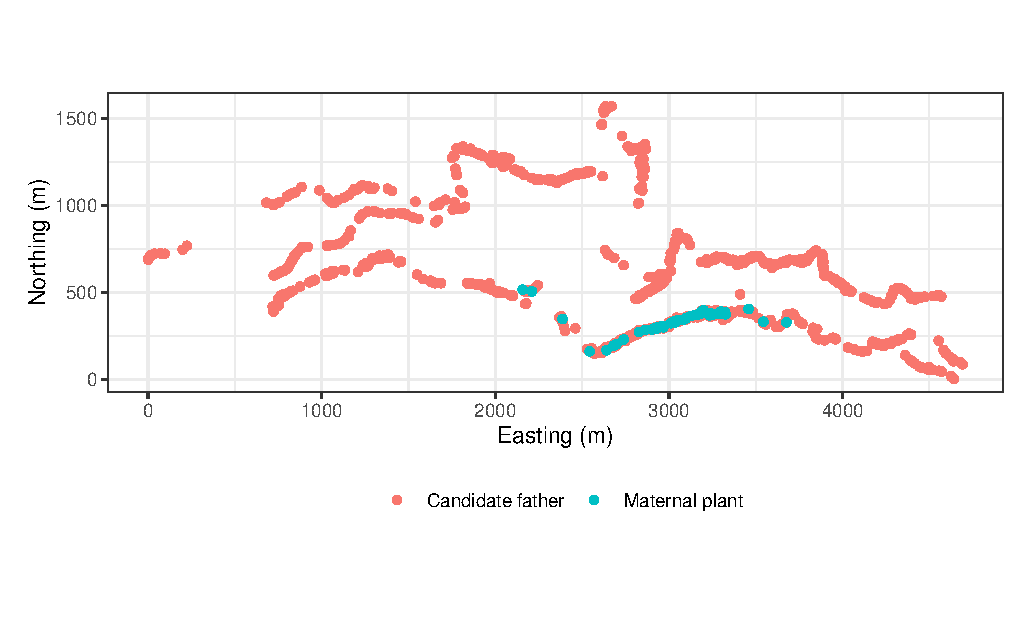
\includegraphics[]{map.eps} % Figure image
	\caption{Map of the hybrid zone. The map shows the distribution of maternal plants and sampled candidate pollen donors along the lower (South) and upper (North) roads.}
	\label{map} % Label for referencing with \ref{bear}
\end{figure*}

We examine a hybrid zone population of the snapdragon \textit{Antirrhinum majus} in the Spanish Pyrenees. Here, the yellow-flowered \textit{A. m. striatum} and the magenta-flowered \textit{A. m. pseudomajus} meet and hybridise to produce diverse recombinant phenotypes, including pink, white and orange flowers.
The population grows along two parallel roads running East-West close to Rib\"{e}s de Freser (figure Fig. \ref{map}). The ’lower’ road is at 1150-1200m above sea level, whilst the ’upper’ road climbs 1250-1500m, and is 500-1000m north of the lower road. Hybrids are mostly confined to a 1km ’core’ hybrid zone, with \textit{A. m. striatum}- and \textit{A. m. pseudomajus}-like plants becoming dominant to the West and East respectively. We surveyed as many flowering plants as we could find in June and July of 2012 (n=2124), and collected information on flower number and location using a Trimble GeoXT datalogger. We collected two to three leaves for DNA extraction and dried these in silica gel (Fischer Scientific). \textit{A. majus} grows in disturbed habitats such as roadsides and railways; they are rare in the established forest and pasture between the two roads, on the north-facing slope to the South, and on the high mountain peak to the North of the two roads. It thus is likely that we sampled the majority of the plants that flowered during the study period, although we cannot exclude that some flowering may have occurred before or after this. 

Pollination is carried out exclusively by large bumblebees and carpenter bees who are large enough to open the flowers \cite{vargas2010occluded, andalo2019prevalence}. \textit{A. majus} has a sporophytic self-incompatibility system, and self-pollinated seeds are very rare.

In August 2012 we collected a single, mature, wild-pollinated fruit from each of 60 mothers (Fig. \ref{map}). In order to minimise disturbance to the population we only sampled from plants which had set a minimum of five mature fruits. These mothers were chosen to represent an even sample of pigmentation genotypes, spread as evenly as possible across the core of the hybrid zone where hybrids are most dense, resulting in 10 \textit{A. m. striatum}-like, 17 \textit{A. m. pseudomajus}-like, and 33 hybrid-phenotype mothers.

\subsubsection{Genotyping}

We grew seeds in 5cm plug trays filled with potting compost (Gramaflor) in a greenhouse under Sylvania GroLux lights on a 16-hour cycle. We sowed three seeds per plug for 50-70 plugs per maternal family and thinned seedlings to a single seedling per plug after cotelydons had appeared. We transferred approximately 1cm2 of fresh tissue from 1419 seedlings to 96-well DNA-extraction plates (LGC Genomics, Berlin) and allowed tissue to dry using the sample bag and silica gel provided. For parental tissue from the hybrid zone we transferred approximately 1cm2 tissue dried in the field to the same plates. DNA extractions of the plated tissue samples were carried out by LGC Genomics.

We genotyped tissue samples at 71 SNPs by KASPR sequencing (LGC Genomics). These SNPs are a subsample of a panel used for a wider survey of the hybrid zone (David Field, unpublished data). The total SNP panel is a mixture of [how many?] diagnostic (showing a gradient in allele frequency) and (how many?) parentage (with as even a gradient in allele frequency as possible) SNPs. Previous work identified the per-locus genotyping error rate  in these data to be approximately 0.0013 (ref?). For parentage loci we chose only biallelic loci with a minor allele frequency greater than 0.3 in each of inner four pools closest to the centre of the cline, selected to be at least 2cM apart. Diagnostic SNPs were either linked to pigmentation loci, or else showed sharp clines across the hybrid zone. We removed 474 offspring and four adults that had missing data at more than 7.5\% of the SNPs. We also pruned 7 SNPs that showed more than 10\% missing data, or less than 15\% heterozygosity. This left us with a set of 984 offspring from 60 maternal families, with between two and 29 offspring per maternal family (mean=16.4).

\subsubsection{Inference of mating events}

We aimed to create a list of possible mating events between mothers and candidate fathers consistent with the data. Since FAPS integrates over a distribution of full sibships, we are agnostic about the absolute number of offspring sired, and focus instead on the probability that a candidate males sired at least one offspring in the sample with a given maternal plant. For each partition structure, FAPS identifies valid combinations of fathers for each full sibship, and estimates a likelihood for each father-sibship configuration by Monte Carlo simulation. Each set of fathers reflects a set of mating events, and the probability that a single father mated with the maternal plant is the sum of probabilities for each partition structure in which he sires at least one offspring. This gives a list of mating events, with a posterior probability that each occurred. Note that because estimates are weighted averages, the number and size of sibships are not necessarily integers.

For 1000 iterations of the MCMC output we inferred mating events in this way, based on genetic information and probabilities of dispersal from the scale and shape values for that iteration in sibship clustering (eqn. \ref{eqn:pairwise_with_covariates} and \ref{eqn:sibship_with_covariates}). This gives 1000 sets of mating events for each iteration of the MCMC output. Because results for different prior dispersal scenarios were very similar we present results for the ‘restricted-kurtosis’ scenario unless otherwise stated.

\subsection{Power analysis}

We used simulations to determine the statistical power of the dataset to identify true fathers, and to compare the power of analyses based on paternity alone, sibship information, and dispersal information. We simulated mating events based on pollen dispersal kernels from the posterior distribution of the “restricted kurtosis” analysis. For each iteration in the chain we simulated mating events between each mother and sires drawn from the pool of genotyped adult plants. We drew sires based on the probability of mating under dispersal parameters for that iteration and simulated offspring genotypes based on Mendelian segregation. For each mother, we simulated as many mating events with the same numbers of offspring as were inferred in the observed data for that iteration. After mating, we simulated genotyping errors to adults and offspring genotypes with probability 0.0013 (the observed genotype error rate) per locus per individual. We simulated one dataset for each of 1000 iterations from the MCMC. In this way simulated data reflects the structure of the empirical dataset.

Given that in the observed data we found that most offspring/sibships had one clear candidate father with a probability close to one we quantified how often the true father of each individual was identified as the top candidate. We did this for matrices of paternity probabilities for each offspring:
\begin{enumerate}
\item Based on paternity probabilities of individuals alone, ignoring sibship and dispersal information.
\item After clustering into full sibships, including both paternity and sibship information.
\item After clustering, including probabilities from the dispersal kernel, which was assumed to be known.
\end{enumerate}
For (2) and (3) we used FAPS to calculate the mean probability of paternity over possible sibship partition structures, weighted by the likelihood of each partition structure, for each individual offspring. In all cases we used a prior probability for the proportion of missing fathers of 0.32. In this way we were able to assess the power to detect a true father for each simulated individual.

\section{Results}

\begin{figure}
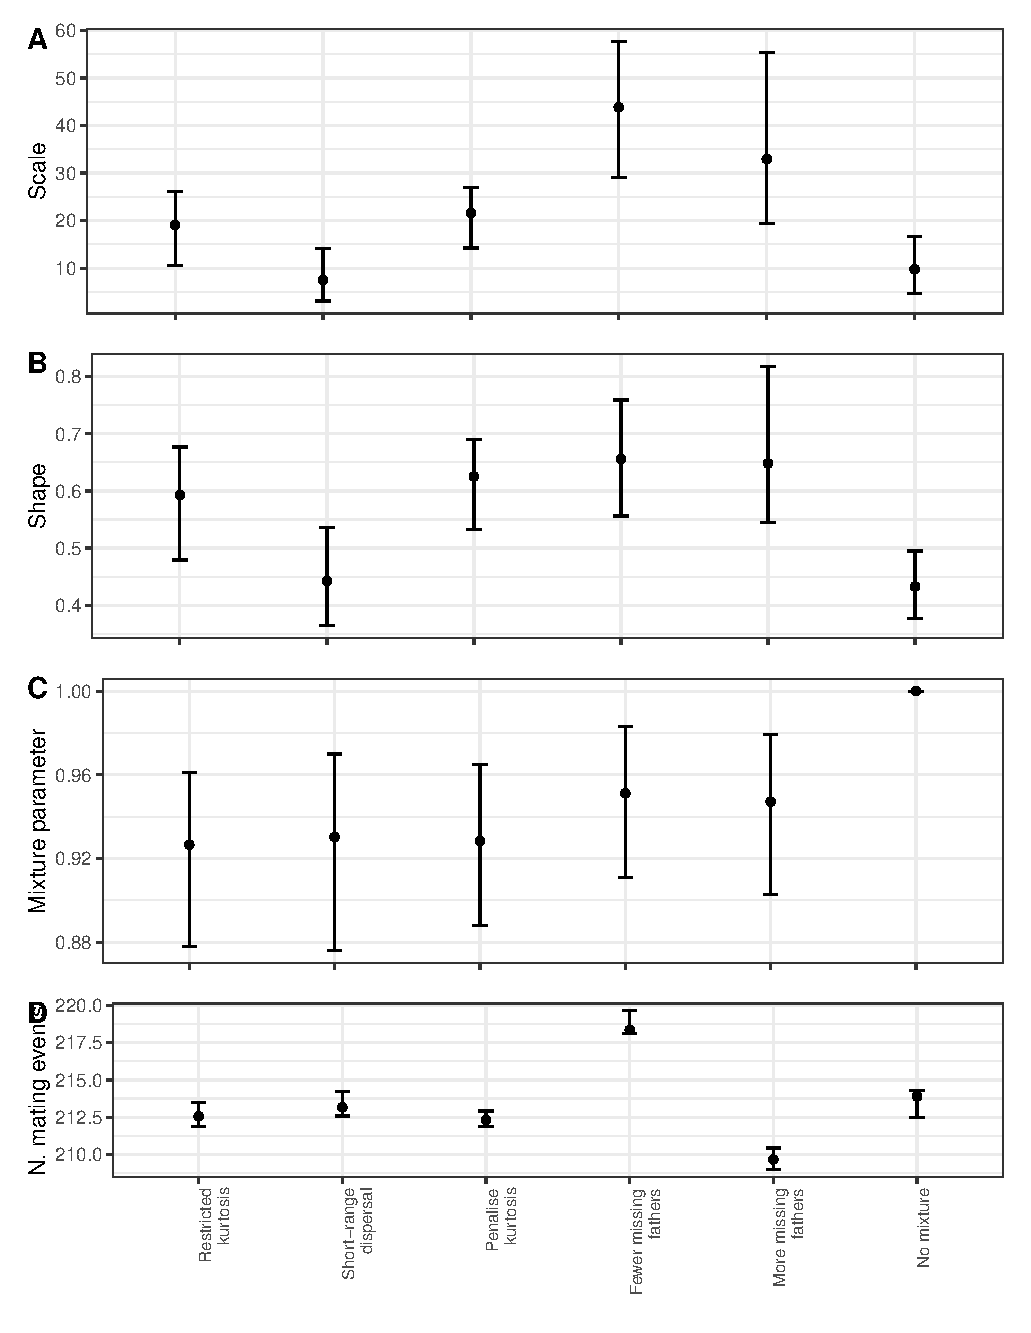
\includegraphics{posterior_distributions.eps}
\caption{Summaries of posterior distributions showing means and 96\% credible intervals.}
\label{posterior_summaries}
\end{figure}

\subsection{At least 200 full sibships}

Across prior dispersal scenarios, independent MCMC chains converged on the stationary and were generally well mixed (Fig. \ref{posterior_summaries}, Fig. SX, SX). The exception is when we set q to 0.42, in which case chains took longer to converge, and tended to become stuck in local optima.

We identified an average of 212.6 (96\% CIs: 211.9, 213.5) full-sibling families for which a father could be positively identified for the ‘restricted-kurtosis’ prior scenario, including 55.5\% of the offspring. Results for the ‘short-range-kurtosis’ and ‘penalise-kurtosis’ scenarios were very nearly identical, and variation in the number of full sibships between prior scenarios was similar to variation within each MCMC chain (Fig. \ref{posterior_summaries}). In contrast, we identified more apparent mating events when the proportion of missing fathers was lowered to 0.22, and fewer when it was raised to 0.42. Prior expectations about the proportion of missing fathers thus had a greater effect on the number of mating events that could be detected than did prior beliefs about dispersal parameters.

We estimated sibship sizes by averaging over parent-sibling configurations, weighted by the probability of each configuration. Focussing on the ‘restricted-kurtosis’ prior scenario, full-sibship sizes varied between less than 1 (indicating that the mating event was only detected for one or more paternity-sibship configurations with very low support) to 20. Averaging over iterations, 96.8\% of offspring were grouped into families of two or more full siblings with one clear candidate father, all with posterior probabilities $\geq$0.999. In contrast, sibships with <2 offspring had much weaker support, with substantial uncertainty about the existence and paternity of those families across the iterations (figure SX). Most offspring thus could be assigned to paternal families with a clear father with high confidence, but caution is needed in interpreting singleton sibships.

The GLM of the number of full sibships on maternal-family size revealed that log number of sibships increased by 0.068 ($\pm0.012$) for every additional offspring included in the maternal family (intercept $= 0.084 \pm 0.250$). This corresponds to detecting a new family for approximately every 3 or 4 offspring genotyped, on average.

For all sixty mothers we found a mating event with non-zero probability for which the father one or more offspring was not sampled, including 44.5\% of the offspring. 93\% of these cases had posterior probabilities $>0.99$. Simulations indicated that the true number of mating events for which the father was not sampled was 108.2 on average (96\% credible intervals: 90, 127). Assuming the number of sampled fathers was 213 (Fig. 2D), this corresponds to approximately 33.6\% missing fathers (96\% credible intervals: 29.7, 37.4).

\subsection{Pollen dispersal is leptokurtic}

\begin{figure*}
    \centering
    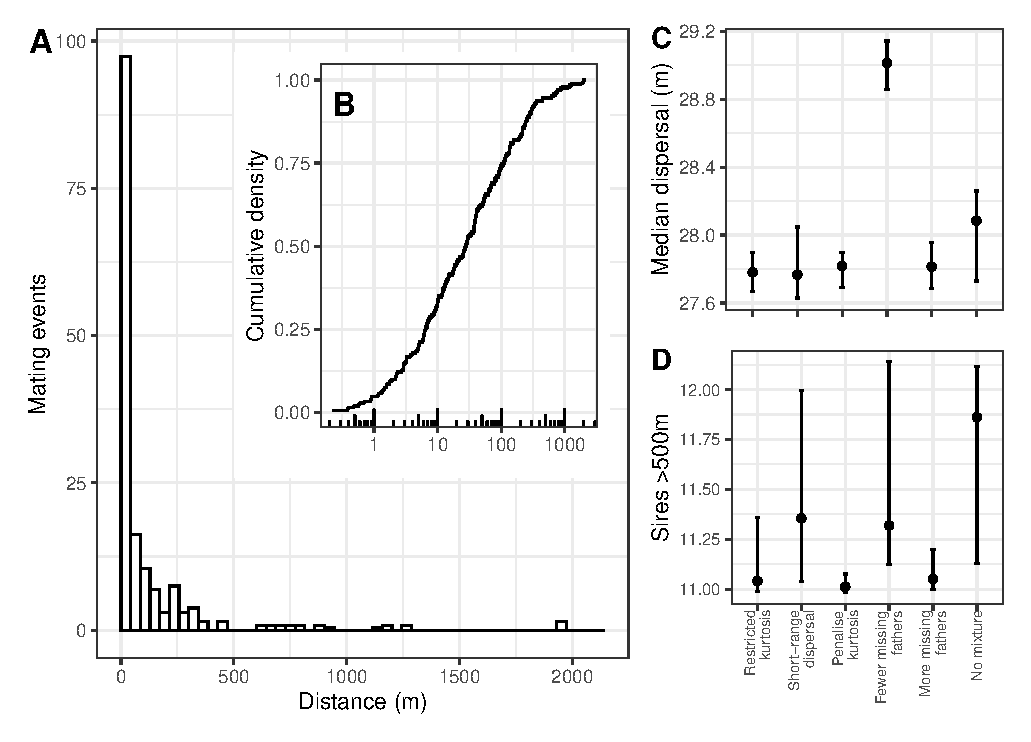
\includegraphics{dispersal.eps}
    \caption{Distribution of pollen-dispersal distances.  (A) Histogram and (B) cumulative distribution of distances for mating events under the “restricted-kurtosis” prior scenario. Note the log10 scale of the x-axis in B. Mating events are weight weighted by their posterior probability. The histogram is summed over iterations of the MCMC. Separate cumulative curves are shown for 1000 MCMC iterations separately. (C) Median dispersal distances and (D) the number of sires more than 500m from the mother across six prior scenarios, showing posterior means and 96\% credible intervals.}
    \label{fig:dispersal}
\end{figure*}

The posterior distribution of both the scale and shape parameters of pollen dispersal varied between prior dispersal scenarios, but in all cases the shape parameter was consistently less than 1 (Fig. \ref{posterior_summaries}, Fig. SX), indicating leptokurtic dispersal kernels. This was true even for the ‘penalise-kurtosis’ prior scenario, which sets essentially zero prior mass on leptokurtosis (Fig. S1). Consistent with this, the distribution of pollen dispersal distances shows a peak close to zero, with a long tail of long-distance dispersal events up to 2102m (Fig. \ref{fig:dispersal}A). Posterior-mean median dispersal under the “restricted-kurtosis” prior scenario was 27.7m, with 25.6\% of dispersal events further than 100m, and 5.0\% greater than 500m (Fig. \ref{fig:dispersal}B). Values for other prior scenarios were very similar; although there were differences in the positions of the posterior distributions, the absolute differences in median dispersal distance and the number of long-distance mating events were small (Fig. \ref{fig:dispersal}C, \ref{fig:dispersal}D). There was very little variation in cumulative dispersal curves across iterations with different dispersal parameters, indicating that there was strong signal from genetic information about the shape of the dispersal kernel (Fig. \ref{fig:dispersal}B). These observations demonstrate that pollen dispersal in this sample was strongly leptokurtic, and that this finding is robust to specification about prior beliefs about dispersal and the proportion of missing fathers.

\subsection{Mixture parameter reduces bias in dispersal shape}

In MCMC analyses where mixture parameter $\lambda$ was allowed to vary, the posterior distributions broadly overlapped with posterior means around 0.93 (Fig. \ref{posterior_summaries}).
The precise interpretation of this number is somewhat obscure, but the fact that this number is close to, but not equal to zero indicates that at least small proportion of sires are missing, and that other non-sires located far from the mother have high probabilities of paternity by chance.
If ignored, this signal would inflate apparent leptokurtosis in the dataset.
Consistent with this, the posterior distributions for the scale and shape parameter in the ‘no-mixture’ prior scenario are shifted downwards compared to the ‘restricted-kurtosis’ (posterior means drop from 20 to 10 and from 6 to 4.5 respectively), which would indicate a more leptokurtic pollen dispersal kernel (Fig. \ref{posterior_summaries}A, \ref{posterior_summaries}B).
This in turn implies a increase in mean dispersal distance (from eqn. \ref{eqn:sd_GND}) from 103.1m to 186.8m.
Fortunately, the effect on realised mating events is small; although the "no-mixture" scenario was associated with a slight increase in both median dispersal and the number of sires further than 500m (Fig. \ref{posterior_summaries}C, \ref{posterior_summaries}D), these differences were very small in absolute terms.
In this instance then, including a mixture component in the dispersal kernel reduces the bias in dispersal shape and apparent mean dispersal distance caused by missing fathers, but this does not have a large enough impact on realised dispersal distances to greatly affect biological conclusions.

\subsection{Including dispersal information improves power to identify fathers}

\begin{figure}
    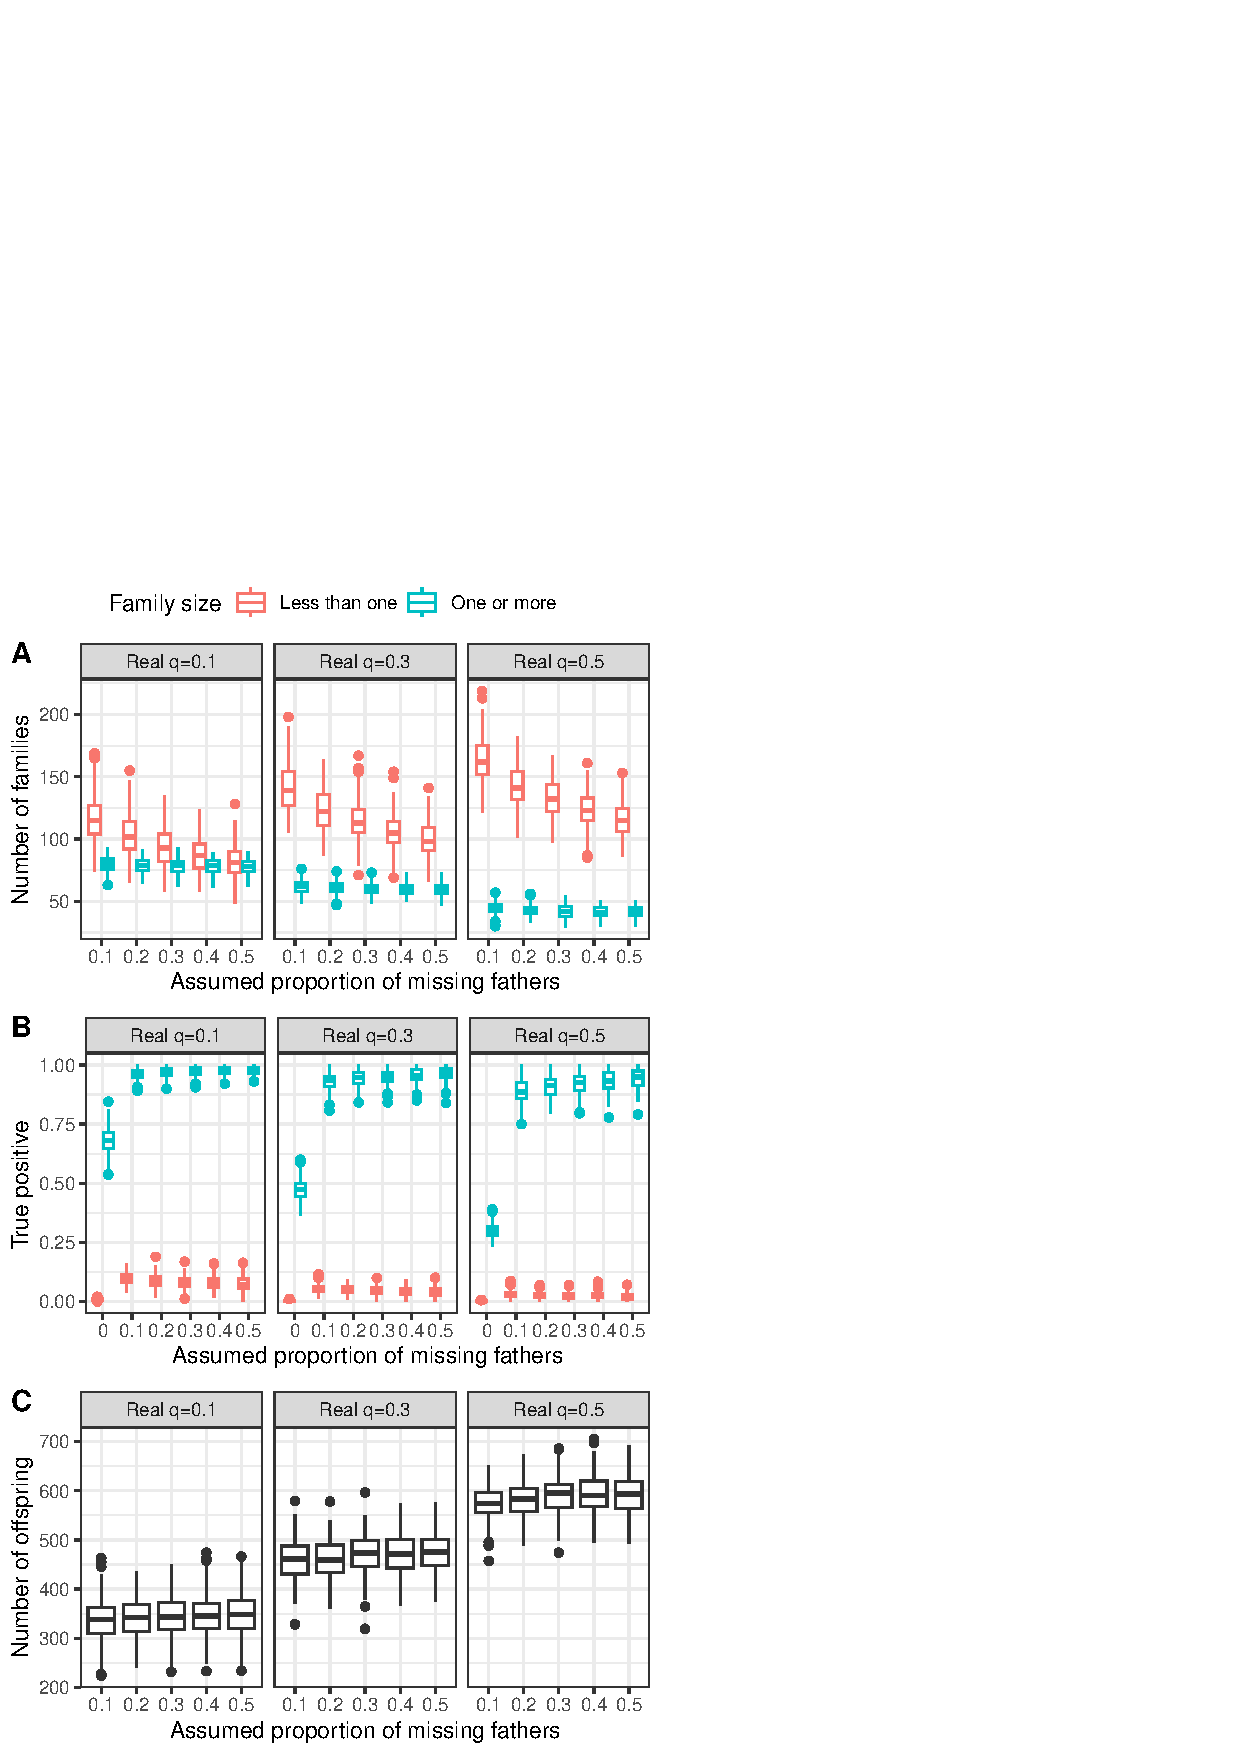
\includegraphics{simulations.png}
    \caption{Simulation results. Plot shows the proportion of individuals for whom the true father was identified with probability $>0.99$ when paternity is inferred based on paternity of individuals only, on paternity and sibship information, and on from paternity, sibship and dispersal information combined.}
    \label{fig:simulations}
\end{figure}

Over 1000 simulations the true father was identified as the most-probable candidate for 90.7\% of offspring when paternity is assessed in the absence of sibship or dispersal information (Fig. 4). This rises to 93.7\% when sibship information is included, and 97.1\% when both sibship and dispersal information are included. This demonstrates the value of performing a joint analysis of paternity, sibships and dispersal, and shows that our dataset has high power to identify the true fathers of individuals.

\section{Discussion}

We have described a framework to jointly infer paternity, sibling relationships and populations parameters. Simulations showed that using all three sources of information leads to a substantial increase in statistical power to identify fathers correctly compared to using paternity, or paternity and sibship information alone. Applying this to a natural populations of snapdragons, we find strong evidence for a leptokurtic pollen-dispersal kernel, which is robust to prior assumptions about dispersal and sampling effort. In the following sections we discuss the implications of dispersal for the population, and caveats and future directions for the method.

\subsection{Comparison with dispersal in other systems}

The results are similar to those found by Field et al. (in prep.) in the same population.
That study used a much large sample of individuals from multiple years and sought to infer the full multiyear pedigree.
The distribution of inter-mate distances is also fat-tailed, with a somewhat higher median distance of X.
This difference in dispersal distances is to be expected.
First, the search space for identifying parents is much larger, because both parents need to be identified rather than just the father, and because parents may have been sampled over multiple years.
Second, although the pedigree is based on more genetic markers, there was no explicit model of dispersal.
Third, the present study considers only a single year; it is likely that the shape and location of the dispersal kernel would vary between seasons.
Despite these differences, the close concordance in results between these two studies indicates that the results are largely replicable.

The finding of leptokurtic dispersal is also consistent with other studies of plant dispersal
A meta-analysis of seed dispersal kernels found that the generalised normal distribution was a good fit for 86\% of datasets examined, and in 87\% of those cases the distribution was leptokurtic.
Fewer studies have been performed on pollen dispersal, but these commonly reported leptokurtic shapes as well (e.g. \cite{adams1992using, austerlitz2004using, robledo2005patterns, klein2008pollen, burczyk2019patterns}, but see \cite{ottewell2012pollen} for a counter example).
All of these studies examined tree populations; to our knowledge ours is the first to estimate dispersal in a non-tree species.

A key difference between this and previous studies of pollen dispersal is that we modelled dispersal as a mixture distribution with a term allowing for false positive fathers that would bias estimates of dispersal.
We showed that using the mixture distribution reduces the bias in the estimated shape parameter and the second moment of the GND, often interpreted as mean dispersal distance.
We note that this bias will exist as long as knowledge of paternity is less than perfect, and as such the mixture model reduces, but probably does not completely eliminate this bias. 
Fortunately our biological conclusions are not affected, because we focus on the distribution of realised mating events, which are affected in only a minor way in real terms (Fig. \ref{fig:dispersal}).
However, caution is warranted in the interpretation of the raw parameter values for shape and mean dispersal from the GND.
It is possible that the effect was stronger here than would be the case in other published studies because our sample of candidate fathers is large, and the spatial extend is much larger (two orders of magnitude) than median dispersal distance.
In contrast, other studies have focussed on wind-pollinated trees, where pollen can travel much further, and with smaller numbers of candidates (e.g. \cite{adams1992using, austerlitz2004using, klein2008pollen}).
This demonstrates the utility of using inferred dispersal parameters to inform inference of real mating events, rather than focussing on the parameters themselves.

\subsection{Implications for the hybrid-zone population}
The shape of the dispersal kernel implies that most mating occurs within tens of metres, but that there is a long tail of mating events between individuals at up to 2 km.

Talk about small stuff - inbreeding

Talk about long stuff
How much pollen could cross the HZ
How does that affect clines


%----------------------------------------------------------------------------------------
%	BIBLIOGRAPHY
%----------------------------------------------------------------------------------------

\printbibliography[title={Bibliography}] % Print the bibliography, section title in curly brackets

%----------------------------------------------------------------------------------------

\end{document}
